\documentclass{mycv}

\newcommand{\CVRole}{senior software engineer}
\newcommand{\CVFields}{autonomous driving, machine learning and artificial intelligence}


\begin{document}
\sloppy % this restricts words spilling out of the margins
\color{templateColor1}
\pagenumbering{gobble}
% \AddToShipoutPicture{\BackgroundPic}

\normalfont
\begin{minipage}[c]{0.32\textwidth}
    %\centering
  %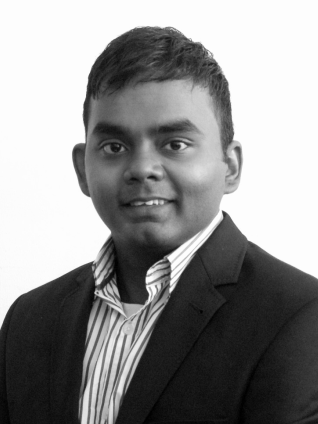
\includegraphics[width=5.2cm]{../img/CV_Photo_comp.png}
  %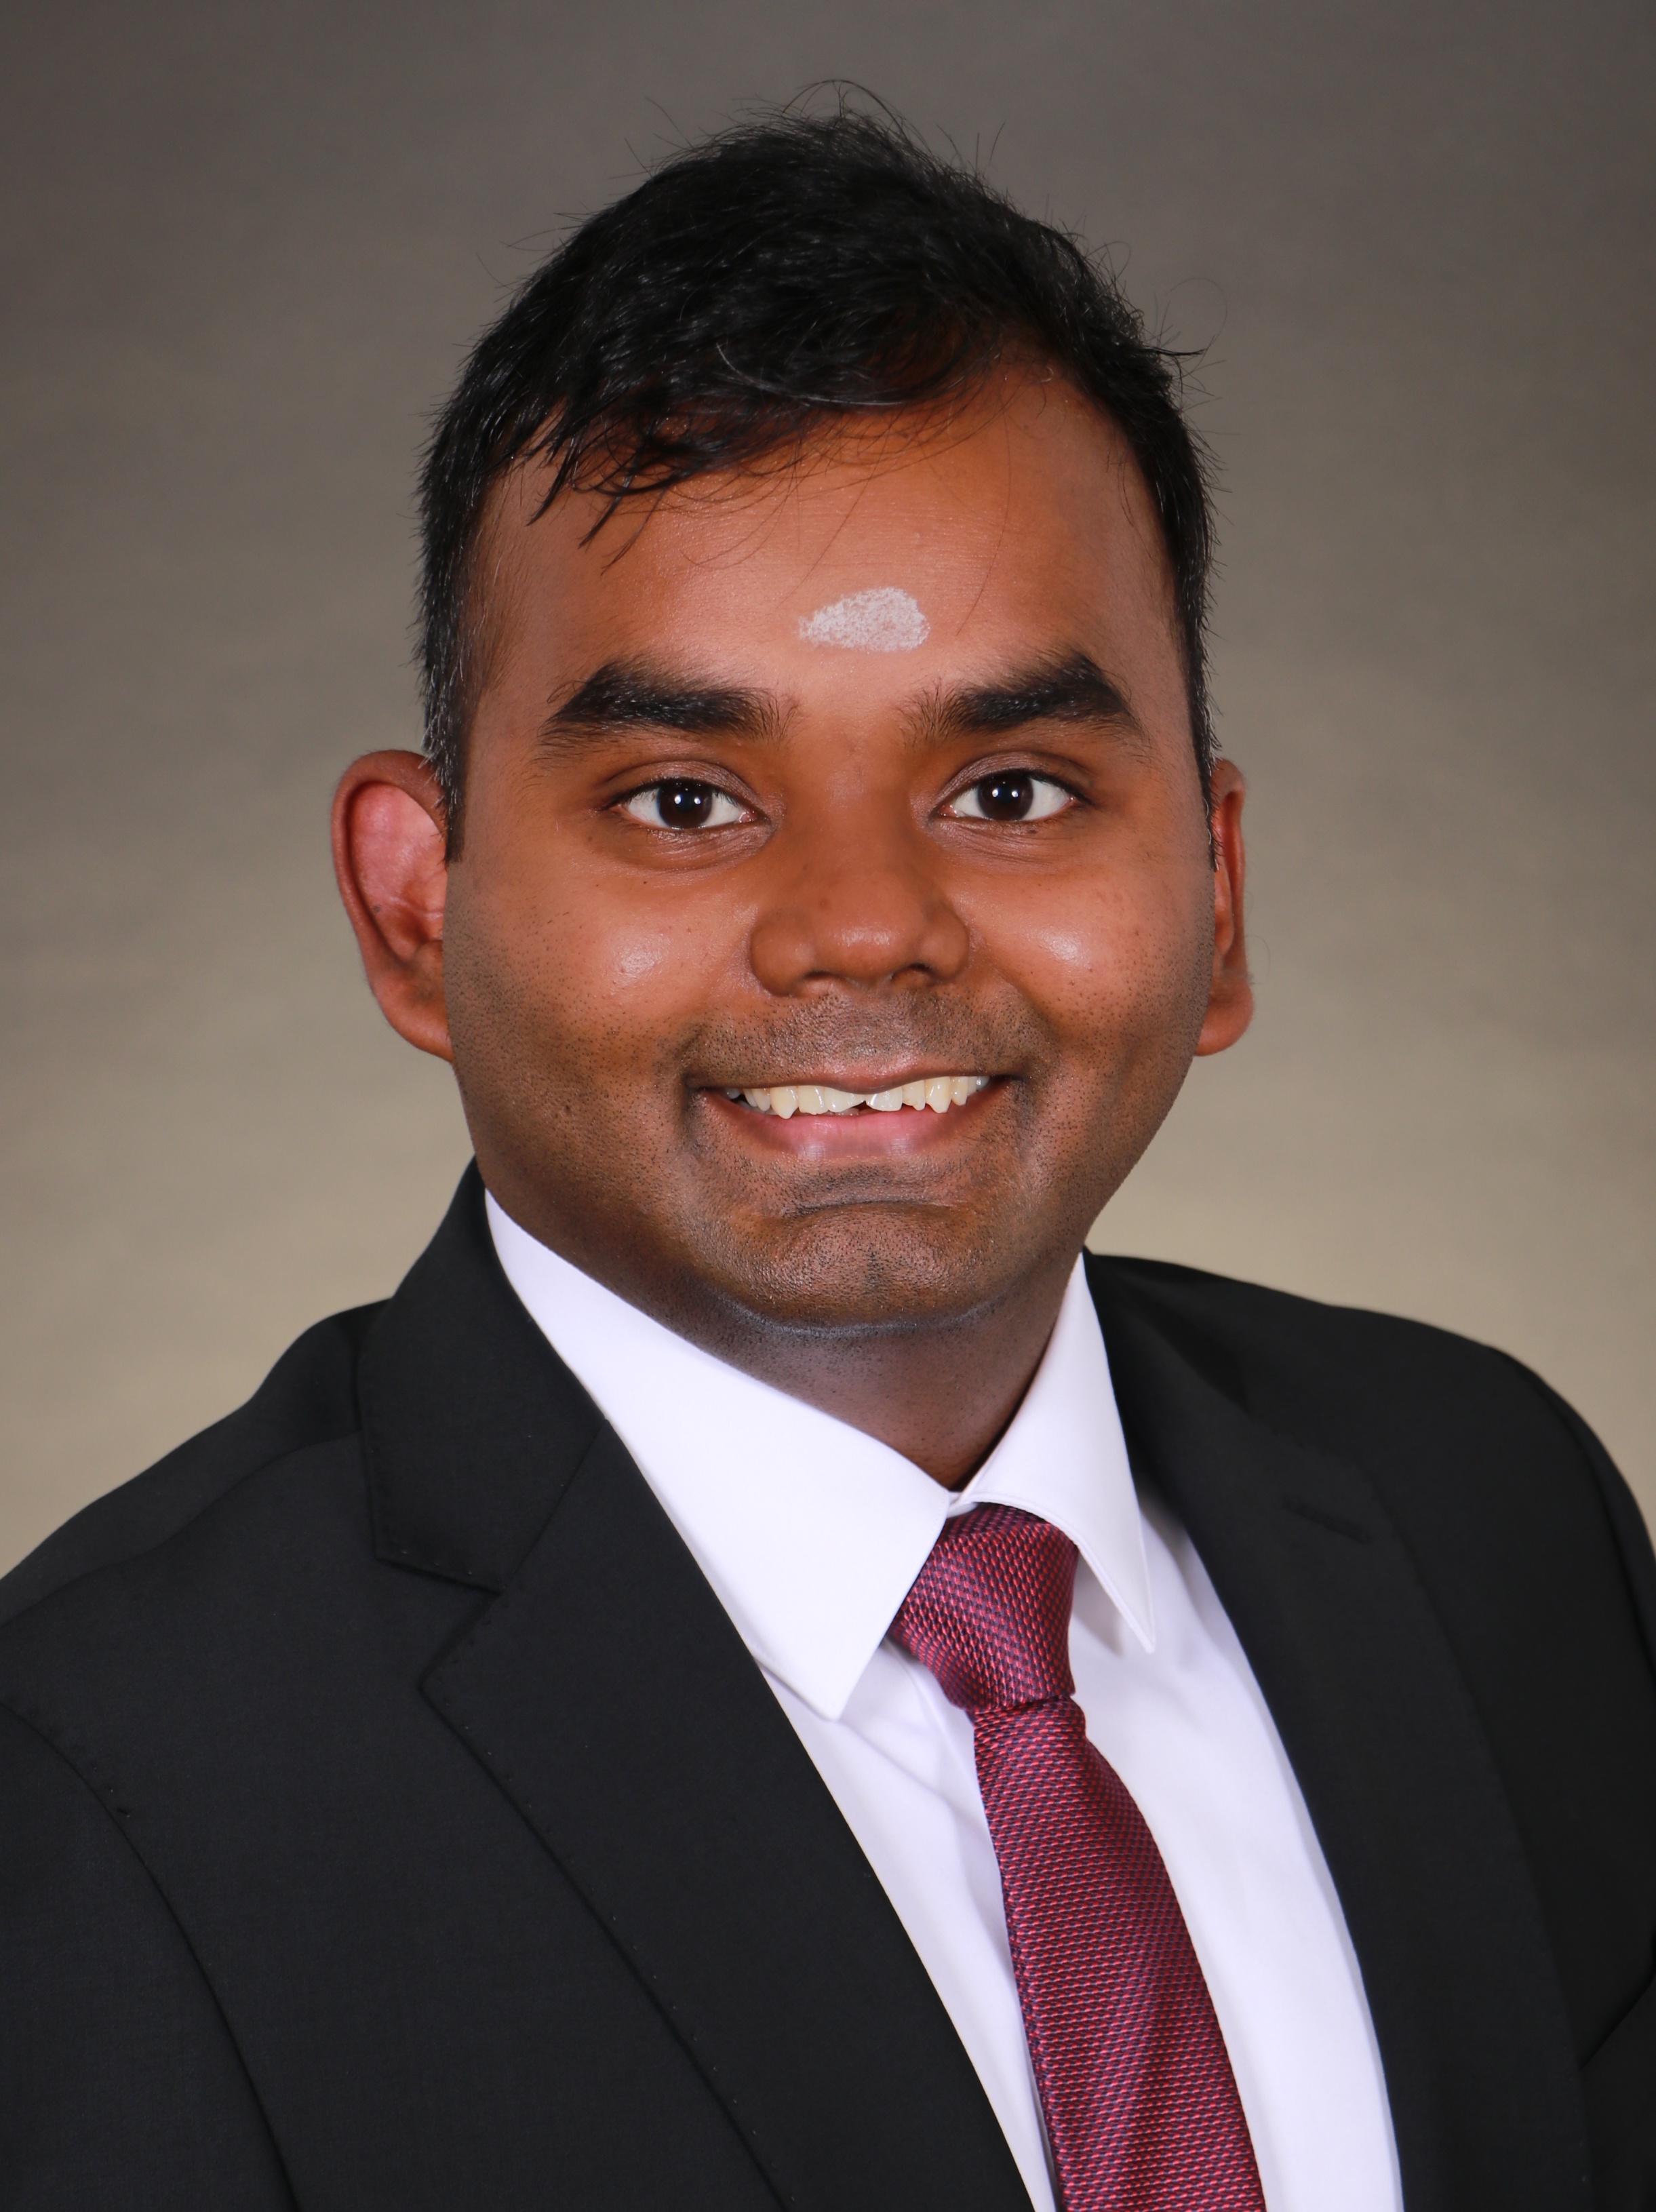
\includegraphics[width=5.45cm]{../img/IMG_7896_m02.jpg}
  % 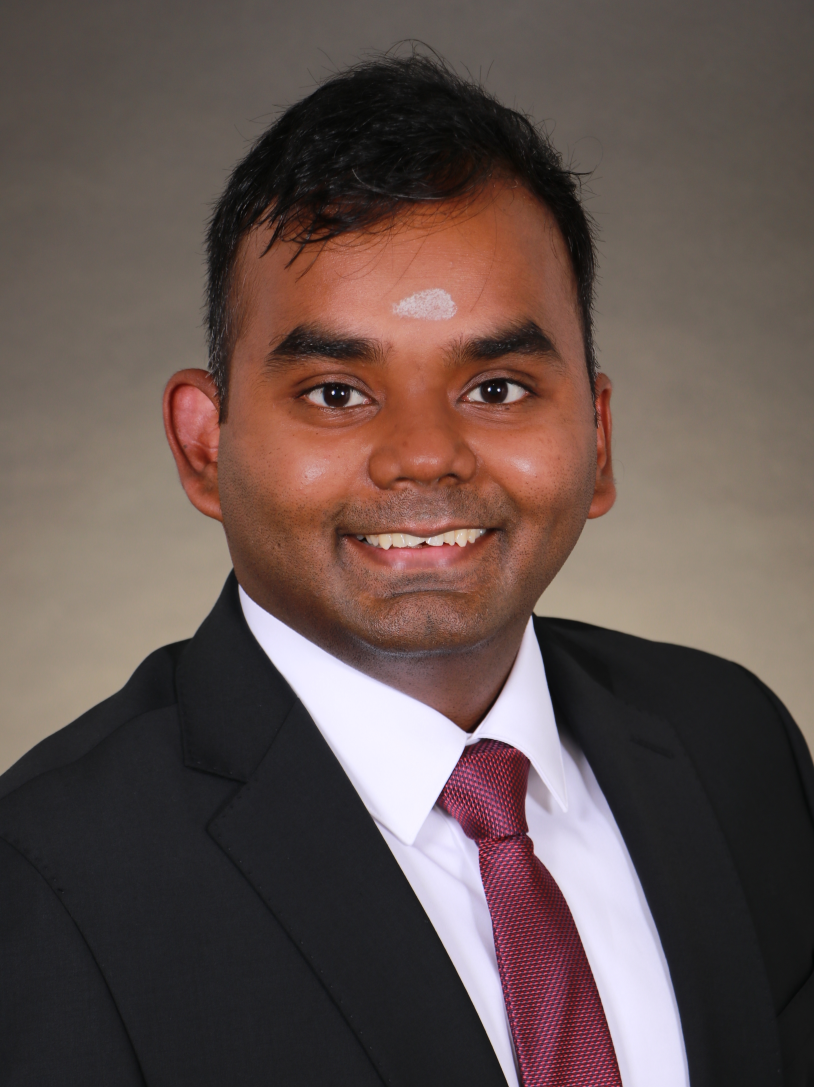
\includegraphics[width=5.45cm]{../img/CV_Photo_new_comp.png}
  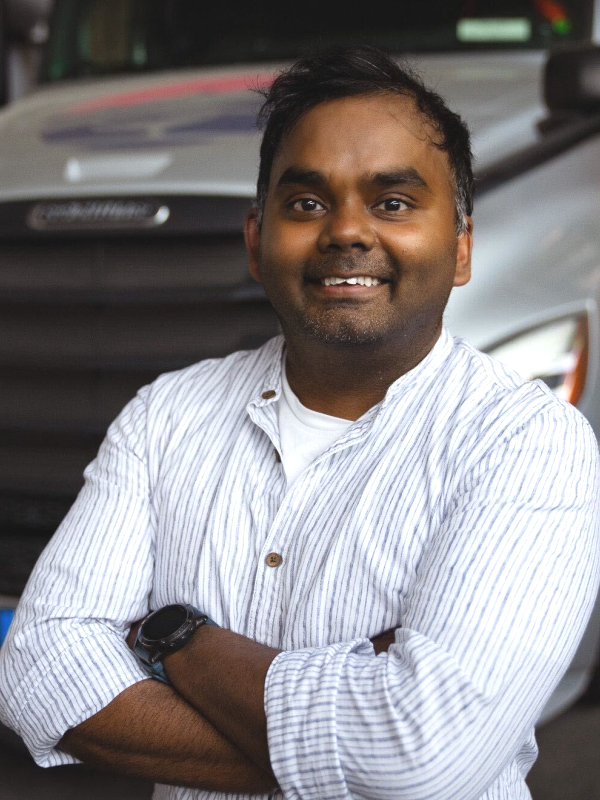
\includegraphics[width=5.7cm]{../img/CV_Photo_Informal_Comp.png}
\end{minipage}
\begin{minipage}[]{0.8\textwidth}

  \vspace{5mm}
      {\huge Dr.-Ing }\\

      {\Huge Chandramouli}\\

    {\Huge Gnanasambandham}
    \vspace{2mm}

    %{\large SIMULATION ENGINEER}
    \vspace{2mm}

  %{\large
    Steinweg 24\\
    71263 Weil der Stadt\\

    \dateOfBirthIcon 6\textsuperscript{th} August 1990\\
  \maritalStatusIcon Married, no children\\
  \telephoneIcon +49 179 6588043\\
  \mailIcon \href{mailto:chandramouli@torc.ai}{\link{chandramouli@torc.ai}}
  %}
  
  \vspace{13mm}
\end{minipage}

{\rlap{\color{templateColor4}\rule[0mm]{\textwidth}{\ulinewidth}}}
\columnratio{0.39}
\setlength{\columnsep}{2.5em}
\setlength{\columnseprule}{\ulinewidth}
\colseprulecolor{templateColor4}
\begin{paracol}{2}
        %\lsection{ANGESTREBTE STELLE}
        % Deutsch #################################################################

        %Ich bin ein leidenschaftlich \,neugieriger
        %Ingenieur mit exzellenten interkulturellen Kommunikationsfähigkeiten. Ich
        %habe 6 Zeitschriftartikel in renommierten Fachzeitschriften publiziert
        %und an mehreren erfolgreichen DFG-Forschungsantr{\"a}gen entscheidend
        %mitgewirkt. All dies war möglich, dank meiner sehr guten
        %Anpassungsf{\"a}higkeit an schnell wechselnden Umgebungen und meiner
        %hervorragenden analytischen, Projektmanagement- und Team-F{\"a}higkeiten,
        %die ich an der Universität erworben habe. Ich suche eine T{\"a}tigkeit als
        %\CVRole, idealerweise im Bereich \CVFields.\\

        % English #################################################################

        \lsection{Profile}

    I am a passionately curious engineer with excellent
    intercultural communication skills. I have been spearheading the
    development of robust multi-fidelity vehicle models for highly-scalable
    simulations with over 300 active users in my current organization.
    Moreover, I have been first author of 6 peer-reviewed journal articles in
    the field of particle dynamics during my time at the academia. All this was
    possible, thanks to my exceptional adaptability to rapidly changing
    environments and my extraordinary analytical and team
    skills. I am now seeking new opportunities as a Senior Engineer,
    where I can leverage my expertise in simulation and analytical
    problem-solving to contribute to cutting-edge innovations in mobility.\\

      \lsection{Languages}
      \begin{doublespace}
            \begin{tabular}{%
                p{2cm}%
                >{\raggedleft\arraybackslash}p{4.5cm}}
            {\mybox\mybox\mybox\mybox\mybox}  &
            {Proficient | German} \\
      {\mybox\mybox\mybox\mybox\mybox} & 
            {Proficient | English}\\
      {\mybox\mybox\mybox\mybox\mybox}  & 
      {Mother tounge | Tamil}  \\
      {\mybox\mybox\mybox\mybox\myboxo}  & 
      {Advanced | Hindi}\\\\
        \end{tabular}
      \end{doublespace}

        \lsection{Web}
        \begin{minipage}[c]{0.31\textwidth}
            \begin{flushright}
                {\bfseries Linkedin}\\
                {\footnotesize
                    \href{https://linkedin.com/in/gnanasambandhamc}{\link{linkedin.com/in/gnanasambandhamc}}}
            \end{flushright}
        \end{minipage}
        \begin{minipage}{0.05\textwidth}
            \linkedinIcon
        \end{minipage}
        \vspace{3mm}

        \begin{minipage}[c]{0.31\textwidth}
            \begin{flushright}
                {\bfseries Medium}\\
                {\footnotesize \href{https://chandramoulig.medium.com}{\link{chandramoulig.medium.com}}}
            \end{flushright}
        \end{minipage}
        \begin{minipage}{0.05\textwidth}
            \mediumIcon
        \end{minipage}
        \vspace{3mm}

        \begin{minipage}[c]{0.31\textwidth}
            \begin{flushright}
                {\bfseries Matlab}\\
                {\footnotesize
                    \href{https://de.mathworks.com/matlabcentral/profile/authors/4267772}{\link{MatlabCentral    Profile}}}
            \end{flushright}
        \end{minipage}
        \begin{minipage}{0.05\textwidth}
            \matlabIcon
        \end{minipage}

\switchcolumn
\rsection{Educational Qualifications}
\subsection{May 2016 - April 2021}{Ph.D. in Mechanical Engineering}
        {University of Stuttgart}\\

        \subsection{October 2012 - April 2016}{Master of Science in Commercial Vehicle
        Technology}{Technical University of Kaiserslautern, {Grade: 1.9}}\\

        \subsection{June 2008 - April 2012}{Bachelor of Engineering in
            Production Engineering}{Anna University, Chennai, India, {Grade CGPA: 8.3/10}}\\

\rsection{Professional Career}
  \subsection{April 2023 - present}{Torc Europe GmbH, Stuttgart}{Staff software engineer}
        \begin{itemize}
          \item Spearheaded a team of four PhDs to design and develop a highly-scalable
              vehicle model in native C++ following Test-Driven Development
              (TDD) and Object-Oriented Programming (OOP)
          \item Integrated vehicle models into a Robotic Operating System (ROS)
              based simulator to enable virtual validation of Level 4
              autonomous vehicles
          \item Partnered with multiple external stakeholders to develop a
              scalable validation strategy for multi-fidelity vehicle models
              following the ISO-26262 standards
        \end{itemize}

  \subsection{August 2021 - March 2023}{Daimler Truck AG, Stuttgart}{Vehicle model engineer}
        \begin{itemize}
            \item Develop multi-fidelity vehicle models for scalable simulations in the context of
        virtual validation in MATLAB/Simulink
          \item Qualify vehicle models following the ISO-26262 standards 
          \item Developed a co-simulation framework to interface a
              high-fidelity multibody system truck model running on a Windows
              client with a virtual driver on an Ubuntu host using TCP/IP
              communication.
        \end{itemize}
\end{paracol}

{\rlap{\color{templateColor4}\rule[0mm]{\textwidth}{\ulinewidth}}}
\begin{paracol}{2}
    \switchcolumn
    \subsection{May 2016 - April 2021}{University of Stuttgart}{Scientific staff at the institute for engineering and
      computational \quad\quad mechanics (ITM)}
          \begin{itemize}
              \item {\bfseries PhD Topic}: Particle Dampers- Enhancing Energy Dissipation using Fluid/Solid Interactions and Rigid Obstacle-Grids
          \end{itemize}
    \subsection{October 2015 - April 2016}{Fraunhofer Institute (ITWM), Kaiserslautern}
        {Intern in the department of mathematics for vehicle engineering}\\

        \rsection{Technical Skills}
        %\begin{singlespace}
        \begin{doublespace}
        %\begin{onehalfspace}
            \begin{tabular}{p{5cm}!{\color{templateColor1}\vrule}p{6.5cm}}
            {\bfseries Programming Languages: } & {\bfseries Operating System:}\\
            {\mybox\mybox\mybox\mybox\mybox 12 years | C/C++}  &
            {\mybox\mybox\mybox\mybox\mybox Linux (Debian, Ubuntu)}\\
      {\mybox\mybox\mybox\mybox\mybox 12 years | MATLAB} & 
            {\mybox\mybox\mybox\mybox\myboxo Microsoft Windows}\\
      % {\mybox\mybox\mybox\mybox\myboxo 9 years | BASH}  & \\
      {\mybox\mybox\mybox\myboxo\myboxo 6 years | Python}  & \\
        \end{tabular}\vspace{4mm}
        \end{doublespace}
        %\end{singlespace}

     {\bfseries Simulation and Data Skills:}
     \begin{itemize}
         \item {\bfseries MATLAB/Simulink:} Modelling, \,simulation,
             numerical optimization, SiL/DiL simulations, MATLAB GUI, FMI
         \item {\bfseries C/C++:} MEX API, SilverBypass, FMI, ROS, TCP/IP and UDP
         \item{\bfseries Multibody-Simulation:}  LMS Virtual.Lab Motion, Neweul-M$^2$, 
             MSC Adams, Project Chrono
         \item{\bfseries ADAS/AD-Simulation Tools:}  Applied Object-Sim, IPG CarMaker, IPG TruckMaker
         \item{\bfseries Multibody-Simulation:}  LMS Virtual.Lab Motion, Neweul-M$^2$, 
         \item {\bfseries Python:} AWS Athena, Ploty Dash, Flask, NumPy, SciPy, Pandas
         %\item {\bfseries Partikelsimulation:} Pasimodo, Project Chrono, DualSPHysics
         %\item {\bfseries Data Visualization:} Paraview, PlotlyDash, Matplotlib, MATLAB 
         \item {\bfseries Other Software Tools:}  Silver Virtual-ECU, COMSOL
             Multiphysics, OptiSlang, Oracle VM VirtualBox
         %\item {\bfseries Sonstiges:} \LaTeX{}, TikZ, Inkscape, MS Office
     \end{itemize}\par

     {\bfseries Software Development Tools:}\par
     \begin{itemize}
         \item {\bfseries CI Tools:} Git, Github CLI, Jenkins, Docker\par
         % \item {\bfseries Development Environments:} \verb|vim|, Visual-Studio Code,
         %     Eclipse \par
         \item {\bfseries Technologies:} PETSc, EIGEN, OpenGL\par
         \item {\bfseries Debuggers/Profilers:} \verb|gdb|, \verb|valgrind|, \verb|calgrind|,
             Intel VTune\\
     \end{itemize}
        

\switchcolumn
      \lsection{Awards}
      {\RaggedLeft \bfseries Best Presentation Award 2014\\}
      Optimization of Vehicle Parameters based on Lap-Time
      Simulations using Multiobjective Evolutionary Algorithm\\

      {\RaggedLeft \bfseries Best Presentation Award 2015\\}
      An Adaptive Approach to Real-Time Estimation of
      Vehicle Dynamics Parameters using Kalman Filtering\\\\
      {\footnotesize Both awards were offered by ALTEN GmbH, complemented
            with a cash-prize of {\bfseries500\,\euro{}} respectively.}\\

    \lsection{Other Fun Projects}
    {\RaggedLeft July 2020 - present\\ \bfseries Raspberry Pi Powered Smart-Home\\}
  As part of a on-going hobby project, I have built a versatile Raspberry-Pi smart home network with remote-ssh-access,
  custom file storage server with automatic backups using \verb|rsync|, Zigbee2Mqtt server for controlling IOT devices
  using siri/google-nest and custom automations.\\

    {\RaggedLeft Juni 2015\\ \bfseries Machine Learning Suite\\}
  Implementation of a deep convolution neural network for optical character recognition as part of a
  freelance software project in MATLAB. To increase performance the {MEX API} was used.\\

    {\RaggedLeft Juni 2014\\ \bfseries Driver-in-the-Loop Simulator\\}
  As part of my work for the KaRaT formula student racing team, I developed a driver-in-the-loop simulator based on
  a communication interface between {IPG CarMaker} and {MATLAB/Simulink}.\\

\switchcolumn
\rsection{Selected Publications}
{\footnotesize
{\bfseries Gnanasambandham}, C.; Fleissner, F.; Eberhard, P.: Enhancing the
Dissipative Properties of PDs using Rigid Obstacle-Grids. 
Journal of Sound and Vibration, Vol. 484, p. 115522, 2020.\\
{\bfseries Gnanasambandham}, C.; Stender, M.; Hoffmann, N.; Eberhard, P.:
Multi-Scale Dynamics of PDs using Wavelets: Extracting Particle
Activity Metrics from Ring Down Experiments. Journal of Sound Vibration,
Vol. 454, pp. 1-13, 2019.\\
% {\bfseries Gnanasambandham}, C.; Sch{\"onle}, A.; Eberhard, P.: Investigating
% the Dissipative Effects of Liquid Filled PDs using Coupled DEM-SPH
% Methods. Computational Particle Mechanic, Vol. 6, pp. 257-169, 2019.\\
% }
\end{paracol}

\begin{figure}[h]
    \begin{picture}(100,50)
        \put(370,0){
\includegraphics[width=5.0cm]{../img/Gnanasambandham_Signature.png}}
    \end{picture}
\end{figure}
\vspace{-0.7cm}\hspace{5.5cm} Stuttgart, \today \quad \hrulefill\\
\raggedleft Dr.-Ing Chandramouli Gnanasambandham

\end{document} 
